\section{Development Plan}

The success of the \grackle{} project as a community resource will depend on
its ability to adapt to the evolving scientific and technical needs of the
users; this development plan has been designed to be responsive to this by 1)
adding features desired by users, 2) encouraging external contribution by
ensuring that the code is easily extendable, and 3) improving performance to
keep up with advances in the simulation codes that use it.
Each year of the work plan has milestones in the form of
deliverables to the community which will enable specific scientific
goals. The features and improvements that we will implement were all
identified in a \grackle{} user survey carried out in Spring 2017 as
being important to the community. In addition, we identify scientific
collaborators with stated intentions of making use of the new features
developed.  Figure \ref{fig:gantt} displays the timeline for the
design, implementation, and delivery of each of the milestones in this
CSSI proposal. In this document, we refer to distinct development plans for
\grackle{} and \dengo{}; the ultimate product of this proposal is a unified set
of software, but we separate them here for clarity.
\grackle{} is distributed under the
3-clause, revised BSD license and has no proprietary
dependencies; all current \dengo{} code will be relicensed from GNU GPLv3 to
BSD 3-clause prior to joining with the existing \grackle{} code base. The
planning and commencement of this work will include direct communication with
the \grackle{} user community via the project's mailing list.

\begin{figure}
\begin{center}
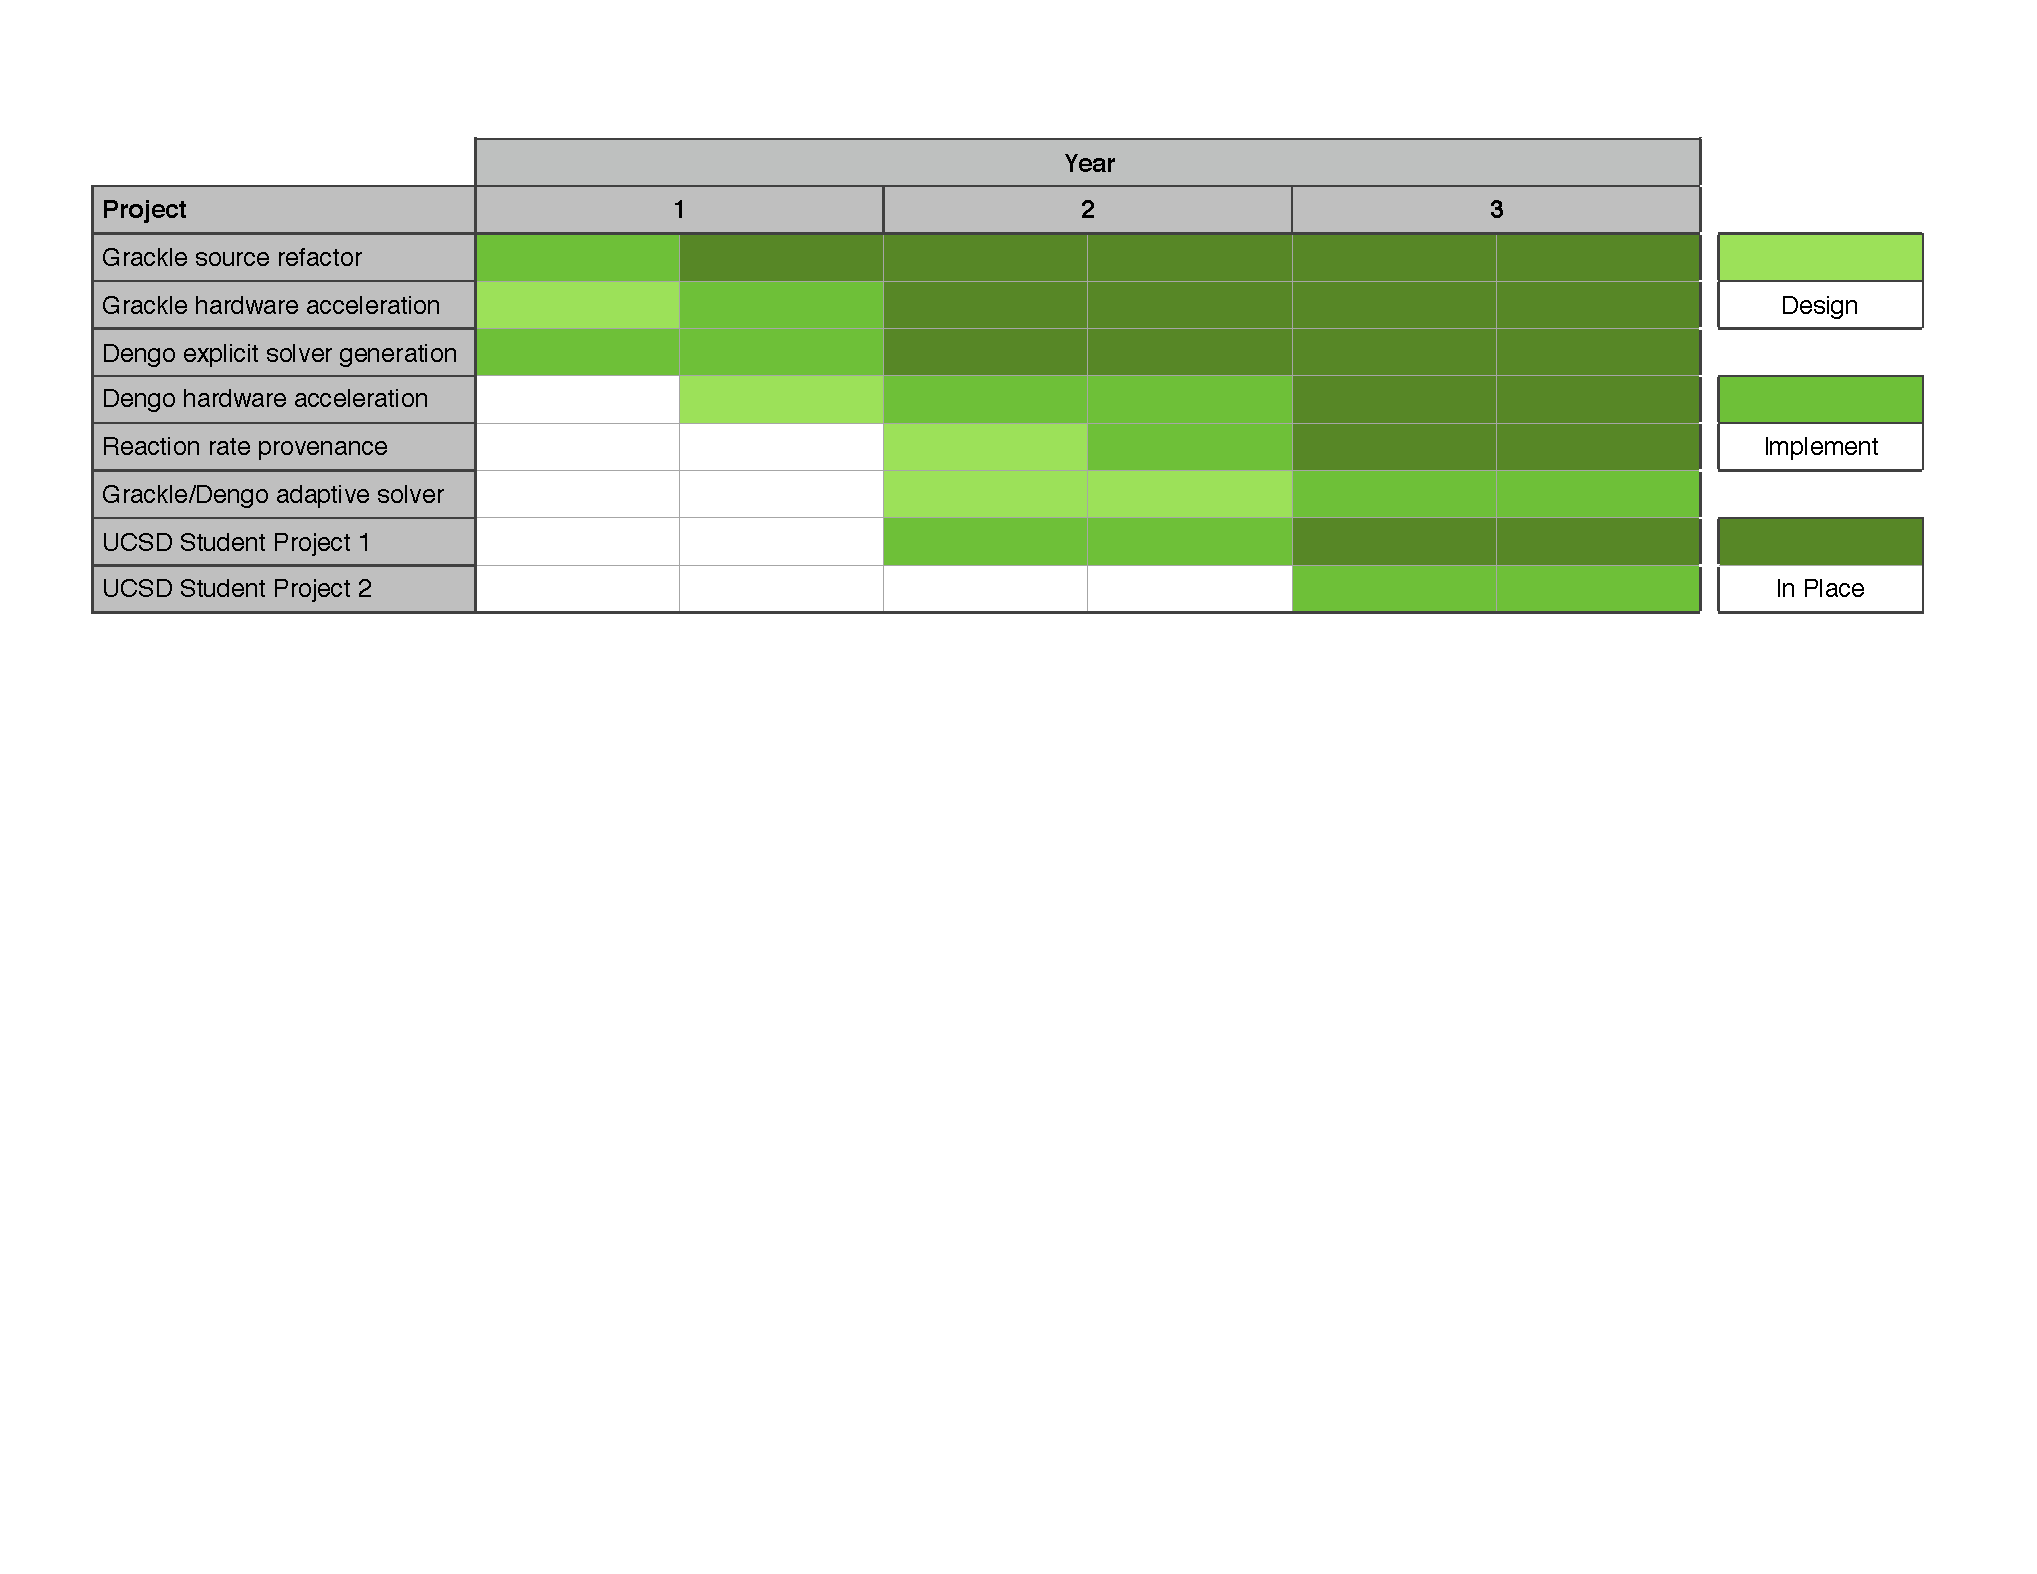
\includegraphics[width=0.9\textwidth]{figures/gantt.pdf}
\caption{Timeline of design, implementation, and delivery of the
  proposed development.}
\label{fig:gantt}
\end{center}
\vspace*{-2\baselineskip}
\end{figure}

The project plan has been devised to provide opportunities for enhancement
while minimizing disruption for community members.  By the end of Project Year
1 (PY1), existing users of \grackle{} will be able to take advantage of hardware
acceleration and \dengo{} will be able to generate (non-accelerated) explicit
solvers with feature parity to \grackle{}.  By the end of PY2, \grackle{} will
be generated using \dengo{} for code generation, and by the end of PY3 the
hybrid explicit/implicit solver will be functional with hardware acceleration.

\subsection{Year One: hardware acceleration and commencement of project unification}

The three objectives for year one are 1) to make \grackle{} subsantially
easier to modify and, hence, more inviting to new contributions, 2)
add generalized support for hardware accelerators to \grackle{}, and
3) to add support for generating explicit solvers to \dengo{}.  The
first two goals will result in a significantly improved \grackle{}
library ready at the end of year one. All three objectives will
contribute to the foundation of the work to be done in years two and
three.

\noindent \textbf{Grackle Source Code Refactor}
The design and optimization of the core chemistry and cooling solver
routines in \grackle{} are central factors in making the library fast
enough to be used in extremely large simulations.  However, these
factors also make this the most challenging area of \grackle{} to
work with as a developer.  For example, to share common data between C and
Fortran, the
Fortran routines must be provided all parameters, fields,
and rate data as function arguments.  This results in intimidating
function signatures with dozens of arguments;
argument inconsistencies result in difficult-to-debug segmentation
faults.
Further complications include maintaining
consistency in variable type across the C/Fortran interface (particularly 32-
and 64-bit) and the
general confusion that can arise from working in two different
languages at once.  
Historically, \grackle{} was written in Fortran to optimize array operation
performance; this speed advantage was especially great when the core solvers
were originally developed in the mid-1990s.  Since that time, advances in the C
programming language, such as the \texttt{restrict} keyword introduced in the
C99 standard \citep{c99}, have made it easier for C code to be competitive
with Fortran.  This will reduce complexity and make the code more inviting to
new developers.

Refactoring \grackle{} will begin by expanding the test suite beyond
the most common running modes and with more fine-grained unit testing.
This strong
testing foundation will enable a safe transition of the Fortran code (roughly
7200 lines) to C.  The resulting code will be vastly streamlined with greatly
reduced function signatures; core routines will be able to access the C
\texttt{structs} containing the run-time parameters, rate data, and field
arrays.  In addition, the ease of calling C routines from Python will allow for
the addition of finer-grained unit tests operating within the existing test
suite, which uses the \texttt{pytest} Python package.  This will also allow for
more of the core functionality to be exposed directly to the user, as has often
been requested.
%% The culmination of this phase of the work plan will be marked
%% by a major public release, \grackle{} version 4.0.

%% At present, on startup \grackle{} computes lookup tables from the
%% functional forms of the reaction rate coefficients.  To enable easier
%% selection, and greater provenance tracking, we will enable the
%% \texttt{pygrackle} wrappers to generate pre-computed tables from
%% functional forms defined in yaml files.  This will provide a method of
%% experimenting with different rates, such as from different
%% experimental results or theoretical calculations, while avoiding the
%% complexity of code generation or full recompilation of the
%% application.  Finally, with this refactor, the
%% increased modularity will allow for the implementation of different
%% solver methodologies.  One potential application of this could be the
%% fully-implicit solver LSODE \citep{LSODE}.  While LSODE is much slower in many
%% cases, it allows the individual to specify a more strict convergence
%% criteria and error threshold than the existing method in \grackle{}.
%% This may provide utility for situations where \grackle{} struggles
%% with time-step convergence, such as at extremely high densities.
%% The result of phase 2 will be a streamlined, more flexible,
%% refactored source code that will be substantially easier to develop
%% and will be released as \grackle{} version 4.0.

\noindent \textbf{Grackle Hardware Acceleration}
As astrophysical simulation codes continue to improve their
scalability and performance, it is important that \grackle{} not
become a limiting factor.  \grackle{}-related calculations are
generally known to constitute 20-25\% of a simulation's computational
cost.  Thus, the potential exists for \grackle{} to serve as a great
help or hindrance to continued performance gains.  Because the
calculations performed by \grackle{} are all local to each fluid
element (i.e., solving a given cell does not require information about
neighboring cells), it was straightforward to achieve modest speedup
with OpenMP simply by threading the outer loops for which the core
functions are called.  However, significantly greater speedups can be
achieved by parallelizing the operations within the solvers and taking
advantage of hardware acceleration options currently available on the
latest high performance computing (HPC) systems, mainly graphics
processing units (GPUs). For example, \citet{Haidar2016PerformanceAA}
report speedups of a factor of 20-40 for an explicit chemistry network
ported to a GPU and even greater speedups when the GPU is used to
compute multiple networks simultaneously.

National computing facilities used for astrophysical simulations, such
as those in the NSF-funded Extreme Science and Engineering Discovery
Environment (XSEDE) and NCSA Blue Waters, employ a variety of
architectures.  Implementing targeted parallelization strategies,
while potentially resulting in faster code, will make the source code
more complex. We will approach this by adopting the well-accepted
OpenACC standard, which supports many different architectures.
OpenACC is supported 
by PGI, Cray, and GNU compilers.  Similar to OpenMP, OpenACC provides
compiler directives, or pragmas, that allow the programmer to
designate portions of code to be run on the
accelerator.  Additional directives provide control of when data is
copied to and from the accelerator and also to allow certain data to
exist only in the accelerator's memory.  This strategy is well-suited
to \grackle{}'s core functions which make use of a number of temporary
variables and data to perform many operations on a series of input
arrays.

Work on OpenACC support will commence immediately following the
refactor of the \grackle{} source code, with the ease of adding
OpenACC support motivating the redesign of the code.  We will
make use of local computing resources at PI Smith's home institution
(San Diego Supercomputer Center, SDSC) for development and testing.
SDSC's Comet supercomputer has 36 NVIDIA dual K80 nodes and 36 NVIDIA
4-way P100 nodes. We will also work with system administrators at
XSEDE facilities to provide modules of pre-built \grackle{}
libraries.
%%  This phase of the project will be released as \grackle{}
%% version 4.1.
Included in this release will be documentation with instructions for
parallelizing new features.

\noindent \textbf{Dengo Explicit Solver Generation and Hardware Acceleration}
As a collaboration between the research groups of PI Turk and PI Smith, during
this year \dengo{} will be instrumented to generate explicit and semi-implicit
solvers.  At present, \dengo{} is able to generate C functions that compute the
Jacobian for a reaction network as well as a consolidated ``right-hand side"
(RHS)
vector that can be provided to solvers such as those in the SUNDIALS suite.
While this enables flexible error control and provides accuracy at
high-densities or in stiff regions of phase space, it is not sufficiently fast
even in those regions where the error introduced from explicit calculations is
low.  This results in behavior that, while fast at high densities (and that
avoid ``ringing" and unphysical oscillations) is unacceptably slow in
low-density regions.

Enabling \dengo{} to output explicit and semi-implicit solvers, such as those
utilized in \grackle{}, will have two primary outcomes: it will enable direct
efficiency and accuracy comparisons with \grackle{} to be made, and it will
enable code generated by \dengo{} to be utilized in \grackle{} itself without
disruption to the broader community.  By experimenting and using the
existing solver mechanism in \grackle{} as a baseline of comparison, the
implementation generated by \dengo{} can be tested, augmented to enable
necessary features (such as detailed reaction-update ordering) and optimized.
Furthermore, as this work will be concurrent with the \grackle{} hardware
acceleration efforts, the two will be conducted in conjunction to ensure that
the explicit solver generated fully meets the standards set by
\grackle{}. Due to the additional complexity of \dengo{}, we will
budget an additional half year in PY2 for the full implementation of
hardware acceleration.

\subsection{Year Two: Reaction Rate Provenance and Model Expansion}

\noindent \textbf{Dengo Reaction Rate Provenance}
Reaction rate coefficients provide the key system for interconnection of a
reaction rate network; these are often determined either via theoretical
calculation or through experimental results.  In many cases, the precise value
to use is not necessarily clear \citep[][see, e.g.,]{2011ApJ...726...55T} and
may also introduce considerable uncertainty into the end-result of a
calculation.  \grackle{} provides primary-literature citations for all of its
rates, as does \dengo{}, but at present the choice of which rate to use (for
instance, to replicate prior results) is not easily accessible.  This limits
the reproducibility of results, as older rates may no longer be easily
accessible, which undercuts the ability of a simulation code to understand
detailed reasons for changes in behavior.  During this phase of the
development, \dengo{} will be instrumented with reaction rate provenance
features.  Similar to the \texttt{citation()} function in R, the output of
\dengo{} will include both the reaction rate solver as well as citations to the
primary literature of the source of each reaction rate coefficient.  This will
be embedded in the solver, in the reaction rates output by the solver, and in
optionally-output text in the initialization step of the solver.  As a
secondary function, \dengo{'s} generation of reaction rate coefficient tables
will be augmented to enable easier toggling of older reaction rates as well as
simplified addition of new reaction rates.

\noindent \textbf{Grackle: UCSD Student Project 1:
  Composition-dependent Metal Cooling Tables}
This project will implement the first of two model-related
enhancements identified in the \grackle{} user survey.
Implementing one of these features is an excellent undergraduate
student project as it has a well-defined endpoint, requires learning
from the scientific literature, provides experience with developing
software for HPC, gives the student recognition within the community,
and allows for the possibility of continued research by working with
the new functionality. In this project, we will expand \grackle{'s}
metal cooling tables from a single
component model that assumes a solar abundance pattern to a
two component system of \citet{2013MNRAS.433.3005D} consisting of
alpha elements (from Type II SN)
and iron-peak elements (from Type Ia SN and intermediate mass stars).
This is a necessary enhancement for new simulations that now treat
multiple sources of heavy elements
\citep[e.g.,][]{2014MNRAS.444.1518V, 2015MNRAS.446..521S}, namely Type
Ia and Type II supernovae and winds from intermediate mass stars.

%% \grackle{'s}
%% current metal cooling tables assume a solar abundance for metals,
%% which has been sufficient for simulations that consider only a single
%% source of metal production, i.e. Type II supernovae (SN). However, recent
%% simulations \citep[e.g.,][]{2014MNRAS.444.1518V, 2015MNRAS.446..521S}
%% now include metal enrichment addition sources, like Type Ia SN
%% and , which produce distinct abundance
%% patterns and associated cooling rates.  In order to support these type
%% of models in \grackle{}, we will implement the method of
%% \citet{2013MNRAS.433.3005D} (updated for the latest UV backgrounds),
%% which consider a two component metallicity 

%%  The goal of refactoring
%% the \grackle{} source code and adding hardware acceleration support is
%% to make \grackle{} an attractive landing spot for external
%% contribution of new chemistry and cooling-related models resulting
%% from scientific research.
%% %% Examples of these include spatially constant models of the evolving UV
%% %% background radiation from stars and black holes
%% %% \citep[e.g.,][]{2009ApJ...703.1416F, 2012ApJ...746..125H};
%% %% approximations for molecular and atomic self-shielding of external
%% %% radiation \citep[e.g.,][]{2012MNRAS.425L..51W, 2013MNRAS.430.2427R};
%% %% and tables of heavy element cooling rates
%% %% \citep[e.g.][]{2008MNRAS.385.1443S, 2009MNRAS.393...99W}.
%% These models are critical to galaxy formation and evolution
%% simulations as they are simplifications of crucial processes that
%% would be computationally prohibitive to calculate directly.  
%% %% Too often, the 
%% %% only publicly available forms of these models are the publications
%% %% describing them, in which important implementation details might be
%% %% omitted.
%% In a survey of \grackle{} users carried out in Spring 2017, a number
%% of such models were identified as features wanted by the community.

\subsection{Year Three: Adaptive Solvers and Model Expansion}

\noindent \textbf{Adaptive solver}
Simulations that span many orders of magnitude in density, straddle different
ionization states and energies and that involve sharp or rapid progression of
boundary conditions (such as supernovae) are particularly challenging for
either fully-implicit or explicit solvers.  In the regions where the stiffness
of the chemical kinetic rate equations is low, the overhead and cost of an
implicit solver is likely too high for efficient computation; in the regions
where the chemical kinetics require tight error control, the usage of an
explicit solver can result in calculations that either take far too long due to
ringing or oscillation or that simply produce incorrect results.  Of particular
concern are situations where some reaction rates are stiff and others are not.
In some instances (notably in the simulation of the first stars in the
universe) the chemical reaction network can become the limiting step at high
densities, but is trivial at low densities.

A number of algorithmic approaches have been developed to address these concerns;
for instance, grouping reaction rates to decrease stiffness and enforce species
conservation in ``chemical families''
\citep{doi:10.1002/kin.550100907, SANDU19973151}, or applying 
asymptotic methods for explicit solvers of stiff networks
\citep{1749-4699-6-1-015001}.  Further approaches such as 
quasi-steady-state (QSS) methods \citep{1749-4699-6-1-015002} and 
partial equilibrium (PE) methods \citep{1749-4699-6-1-015003} may provide
additional opportunities for fast and accurate adaptive approaches.

During PY3, the research teams of PIs Smith and Turk will implement these
methods within the joint framework.  This is a crucial capability that is
fundamentally unavailable at present to computational astrophysics
calculations; the flexibility of modifying the templated, semantically-aware
output from the \dengo{} infrastructure while still providing the consistent,
well-utilized API from within \grackle{} will dramatically broaden the problems
to which this unified software package can be applied.  By providing multiple
layers of abstraction from the underlying implementation, solvers can be tuned
based either on information available to the individual generating the solver
or to heuristics available from the reaction rates themselves.  At the
conclusion of PY3, the unified framework will be able to provide comparative
diagnostics of efficiency and accuracy for mixtures of algorithms for chemical
families, asymptotic approaches, QSS and PE methods, enabling researcher to
make informed decisions about their algorithmic choices without requiring the
overhead of creating a full reimplementation.

\noindent \textbf{UCSD Student Project 2: Metal Cooling
  Tables for Radiation Hydrodynamics}
Due to the expense of radiation transport, simulations have
traditionally modelled the radiative feedback from stars with the
injection of additional thermal energy into the fluid.  Increasingly
simulations have been able to include radiation
hydrodynamics \citep{2012MNRAS.427..311W, Xu_2013, Wise_2014,
2015ApJ...807L..12O}, which has allowed for more accurate treatments of the
radiative component of stellar feedback.  These simulations
still only account for the radiative heating of primordial elements, H
and He, and heating of the metals has been notably ignored, which can
lead to significant over-cooling \citep{2011MNRAS.413..190T,
  2012MNRAS.427..311W}.  This project will create
metal cooling tables specifically designed for this new generation of
radiation hydrodynamics simulations.  We will use the \texttt{Cloudy}
photoionization code to produce cooling tables resulting from the
radiation of simple stellar populations.  These tables will allow for
more accurate calculation of thermal properties of the interstellar
medium due to local stellar sources.

%% \textbf{Science Enabled:}

%% THIS TEXT IS OLD BUT MIGHT BE REUSABLE

%% The goal of the year three development project is to expand the user
%% base of \grackle{} to include the present-day star formation
%% community.  
%% In contrast to the early Universe, where only H$_{2}$ is important,
%% star forming clouds in the local Universe are governed by a host of
%% additional processes, including heat input from cosmic rays and nearby
%% stars; cooling from molecules like CO, OH, and H$_{2}$O; cooling from
%% atomic C/O fine-structure emission; and both heating and cooling
%% effects from dust grains.  Following the detailed chemical structure
%% of these complex environments is currently outside the range of
%% \grackle{}'s capabilities.  However, detailed studies of the minimal
%% chemistry networks required for accurately modeling these systems
%% \citep{2012MNRAS.421..116G, 2017ApJ...843...38G} have paved the way
%% forward.  Expanding the chemistry solver to include additional species
%% will help to significantly grow the community of \grackle{} users.
%% This expansion was also the number one requested feature (by 16 out of
%% 23 total respondents, representing 9 of the supported codes) in a
%% recent online survey of current \grackle{} users.

%% In year three, the existing primordial chemistry network will be
%% expanded to include the network of \citet{2017ApJ...843...38G}.  This
%% is an 18-species network that includes O, O$^{+}$, C, C$^{+}$, CO,
%% HCO$^{+}$, Si, Si$^{}$+, CH$_{x}$ and OH$_{x}$ (CH$_{x}$ and OH$_{x}$
%% are pseudo-molecules representing multiple molecules) in addition to
%% the species currently covered by \grackle{}.
%% \citet{2017ApJ...843...38G} show that this network out-performs all of
%% the minimal models discussed in \citep{2012MNRAS.421..116G} when
%% compared to the results of a more sophisticated photo-dissociation
%% region calculation.  The improvements made in years one and two will
%% make this effort significantly easier than if it were undertaken
%% first.  This will also provide a clear path for implementation of
%% additional networks in the future.  The year three project both adds
%% functionality and provides a template for user contributions.

%% This model will be added to \grackle{} using the parallelization
%% strategy implemented in year two and will be released as a 5.x version
%% of the \grackle{} library.

\subsection{Engineering and Release Process}

The \grackle{} project follows an established model for development
and releases that is primarily modelled after that of the \yt{}
community.  The \yt{} project has similar aims as a cross-platform
library for simulations and the PIs have played integral roles in
growing  its community and crafting its governance model.
\dengo{} will emulate this model. The \grackle{}
project maintains a Community Code of Conduct and Developer Guide
to promote a diverse and inviting community.

The \grackle{} and \dengo{}
source code repositories are hosted on
BitBucket.org\footnote{\url{https://bitbucket.org/grackle/grackle} and
\url{https://bitbucket.org/dengo-project/dengo}} and are publicly
readable. PIs Smith and Turk have recently participated in the
transition of other projects to Github and will evaluate such a
transition early in this project. Development proceeds via a ``Pull Request''
(PR) model that allows for incoming changes to be effectively
peer-reviewed before being merged.
Experienced developers are granted write-access to the repo and can
merge a PR once consensus has been reached.
These experienced developers also act as release managers for stable
releases. \grackle{} uses semantic versioning to provide clear
indicators of backward incompatible changes, new features, and bug fixes.

%% \grackle{} is developed using the Mercurial distributed version
%% control system.  The main repository on BitBucket.org is publicly
%% readable with write-access currently granted to a handful of the most
%% experienced developers.  The Pull Request model is used even by those
%% with write access to the main repo.  In this model, a contributor
%% ``forks'' the main repository, commits changes to their fork, and then
%% submits a PR allowing other developers to review the
%% line-by-line changes.  Reviewers leave comments or ``approve'' the
%% PR and it is eventually accepted or declined in a process
%% analogous to peer-review for publications.  At the present time, this
%% usually proceeds with the lead developer (PI Britton Smith) serving as
%% PR manager by identifying appropriate reviewers (including
%% himself) and soliciting comments.  As the community continues to grow,
%% this role can become codified and rotated amongst multiple people.
%% \grackle{} has received 76 PRs since the first release.

\grackle{} contains a suite of unit and answer
tests that can be run manually using the \texttt{pytest} package.  The
test suite runs automatically on the central repository and its
forks using the Bitbucket Pipelines continuous integration service.
The test suite includes a variety of ``unit tests`` to ensure against
violation of fundamental contraints and ``answer tests`` to prevent
results from drifting. The test suite will also compile and
run all code examples and sample scripts.

%% The test suite
%% includes a variety of different tests to guard against regression.
%% Several ``unit tests'' exist to ensure that fundamental
%% constraints are not violated.  For example, the cooling rates should
%% match for identical fluid containers that have different internal unit
%% systems or are in different cosmological reference frames (i.e.,
%% comoving or proper).  \grackle{} also has a series of ``answer
%% tests'', wherein the results of specific calculations are compared
%% against stored values from prior versions.  Finally, to ensure that
%% the library continues to function as advertised, the test suite
%% attempts to compile and run the example codes that demonstrate the
%% APIs.

%% \grackle{}'s documentation is included in the source and is written in
%% reStructuredText, which can be converted to HTML and PDF formats
%% using the Sphinx package.  An HTML rendering of the documentation is
%% also hosted on
%% readthedocs.org\footnote{\url{https://grackle.readthedocs.io}},
%% and is automatically rebuilt when changes are added to the main
%% repository.


\subsection{Provenance and Reproducibility}

Reproducibility is integral to the scientific process, but can be
difficult to achieve when a calculation relies on a complex software
stack where dependency versions change frequently
\citep{2014arXiv1412.5557J, 2016arXiv161009958L}.
%% Increased
%% community involvement in a project, quickening the churn within the
%% source code, only exacerbates the situation.
In \grackle{}, this
problem is solved by building unique version identifiers directly
into the library.  When the library is compiled, the Mercurial
changeset hash (which is effectively unique) is baked into a routine
that outputs relevant information into a sidecar file created at run
time. Included in this file are: a ``diff'' of any uncommitted
changes made to the source, the release
version, all compilation options, and all run-time parameters.
Additionally, \grackle{} maintains a ``CITATION'' file within the
source and in the documentation describing the proper citation
language and BibTex entries to the citable entities.  We will also
follow external examples, where appropriate, to produce machine
readable provenance information \citep[e.g.,][]{force11,
  Fenner097196}.
%% In these ways, \grackle{} serves as an example to
%% the community of mechanisms for making reproducibility documents.

\subsection{Alternative Software Packages}

While the astrophysical literature is replete with descriptions of chemical
reaction networks, other than \grackle{}, there are essentially \textit{no}
cross-platform chemistry and cooling packages packages aimed at large
simulations available to the astrophysical community.  This fact was the primary
motivator for \grackle{}'s creation.  The main alternative to \grackle{} is the 
\texttt{KROME} package
\citep{2014MNRAS.439.2386G}.  \texttt{KROME} is functionally very
similar to \dengo{} in that it can generate implicit solver code for a
user-defined network.  \texttt{KROME} also exposes a number of
distinct chemical networks through a Fortran-based API.  However, this
API varies for each network, so a user must add support for them
individually.  Additionally, \texttt{KROME} is designed exclusively as
a chemistry network solver and so does not employ cost-saving
simplifications, like tabulated metal cooling and self-shielding
models, designed to work in regimes where direct network solving is
computationally prohibitive.  This is an important point as these
methods are widely used in the galaxy formation simulation community.
Finally, \texttt{KROME}'s solvers are designed to operate on a single
fluid element (impeding SIMD-related optimizations) and do not offer additional
parallelization; \texttt{KROME} is not specifically targeted toward large
simulations or advancements in hardware acceleration.

Several codes exist for solving specific chemistry
networks on single fluid elements, such as 
\texttt{ALCHEMIC} \citep{2010A&A...522A..42S}; \texttt{ASTROCHEM}
\citep{2013MNRAS.431..455K}; \texttt{ASTROCHEM} \citep[][unrelated to
the first \texttt{ASTROCHEM}]{2013A&A...559A..53M}; \texttt{NAHOON}
\citep{2012ApJS..199...21W}; \texttt{RATE13} \citep[associated with
  the UMIST database][]{2013A&A...550A..36M}; and \texttt{XDELOAD}
\citep{2005Ap&SS.299....1N}.  \texttt{ASTROCHEM}
\citep{2013A&A...559A..53M} is the only code hosted in a
publicly-viewable repository.  \texttt{NAHOON} and \texttt{RATE13} are
downloadable as tatic tar files.  \texttt{ALCHEMIC} and
\texttt{XDELOAD} are available upon request.  \texttt{ASTROCHEM} by
\citet{2013MNRAS.431..455K} is a private code.
In addition to the above codes, a number of works have provided tables
of cooling rates \citep{1993ApJS...88..253S, 2009MNRAS.393...99W,
2013MNRAS.434.1043O} that require the surrounding machinery for
interpolating and updating the internal energy to be implemented
independently.
These codes and tables supply important functionality, but it is
not their aim to provide a flexible API to large simulations, nor to
act as a two-way resource that both serves and invites contribution
from the larger community.

%% The \grackle{} project has focused on providing optimized, easily
%% adoptable functionality that is independent of simulation code
%% design.  Through its interoperability with other cross-platform
%% astrophysical tools like \yt{}, it seeks to exist within the
%% ecosystem of scientific software rather than alongside it.  The
%% \dengo{} code will adhere to this same philosophy.
%% \grackle{'s} focus on usability, performance, and community
%% involvement make it a vital software element to the field of
%% computational astrophysics.  This focus is underscored by the goals
%% of the work outlined in this proposal:
%% to make the code inviting to new contribution; to enhance performance
%% to scale with next-generation simulations; and to add features desired
%% by its current users as well as to make it useful to new communities.

\subsection{Advisory Board}

We have formed an advisory board to ensure that the milestones
outlined in this proposal are accomplished on schedule. The PIs will
meet regularly (via video-conference) with the full board to present
updates on progress, both technical and toward the overall goals of
the project in terms of growth in users and community involvement.
The advisory board provides a range of scientific and technical
expertise as well as experience with community software development.
%%   The
%% advisory board members are experts in the fields of computational
%% astrophysics and astrochemistry and have significant experience in the
%% development (both technical and social) of community software projects
%% and in parallelizing codes for GPUs.
{\bf Prof. Greg Bryan} is the original author of the \texttt{Enzo}
simulation code and provides experience with chemistry solving methods
and design of large software projects.
{\bf Dr. Anshu Dubey} was an associate director of the Flash Center
for computational science and one of the lead developers of the
\texttt{FLASH} simulation code \citep{2000ApJS..131..273F,
  2009arXiv0903.4875D}.%%   Dr. Dubey brings expertise in developing
%% large adaptive mesh-refinement codes and can advise on adding
%% \grackle{} support to \texttt{FLASH}.
{\bf Dr. Simon Glover} is a foremost expert in astrochemistry and
chemical networks and has contributed numerous updated chemical rates to
\grackle{}.
% %Dr. Glover will provide expertise in creating chemical
%% networks and evaluating their scientific applicability.
{\bf Prof. Michael Norman} is the head of the San Diego Supercomputer
Center and has coordinated development of \texttt{Enzo} and
\texttt{CELLO}/\texttt{Enzo-P}, a peta-scale AMR framework and
simulation code.
%% Prof. Norman provides experience in software design for
%% high performance computing and accelerating codes with GPUs and MIC
%% systems.
{\bf Prof. Stella Offner} is an expert in simulations of present-day
star formation and provides insight into the needs of that community.
Prof. Offner will also advise on adding support for \grackle{} to the
\texttt{ORION} simulation code \citep{2012ApJ...745..139L}.
{\bf Prof. Dan Reynolds} is an expert in developing highly scalable
numerical solvers and an original contributor to \dengo{}.
%% Prof. Reynolds will provide valuable insight into algorithm design and
%% implementation.

%% The advisory board provides a range of scientific and technical
%% expertise as well as experience with community software development.
%% Their input will help to see that milestones are met and that
%% the project satisfies the needs of the communities it seeks to serve.
